\documentclass[tikz,border=6pt]{standalone}
\usepackage{amsmath,amssymb}
\usepackage{tikz}
\usetikzlibrary{arrows.meta,positioning}

\begin{document}
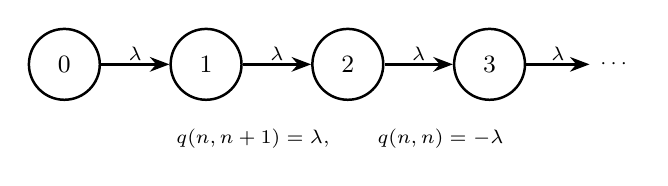
\begin{tikzpicture}[
    >=Stealth,
    line width=0.9pt,
    state/.style={circle, draw=black, minimum size=9mm, inner sep=0pt, font=\small},
    edge label/.style={font=\scriptsize, fill=white, inner sep=1pt},
    note/.style={font=\scriptsize}
]
    \node[state] (0) at (0,0) {$0$};
    \node[state] (1) at (1.8,0) {$1$};
    \node[state] (2) at (3.6,0) {$2$};
    \node[state] (3) at (5.4,0) {$3$};
    \node[note] (dots) at (7.0,0) {$\cdots$};

    \draw[->] (0) -- node[edge label, above] {$\lambda$} (1);
    \draw[->] (1) -- node[edge label, above] {$\lambda$} (2);
    \draw[->] (2) -- node[edge label, above] {$\lambda$} (3);
    \draw[->] (3) -- node[edge label, above] {$\lambda$} (dots);

    \node[note] at (3.5,-0.95) {$q(n,n+1)=\lambda,\qquad q(n,n)=-\lambda$};
\end{tikzpicture}
\end{document}
